\section{Fourier-Transformation}{120}

Im Gegensatz zu den Fourier-Reihen, welche ausschliesslich periodische Signale 'verarbeiten' können, beschäftigt sich die 
Fourier-Transformation mit \textbf{nicht-periodischen Signalen!}


\subsection{Existenz des Fourier-Integrals}{131}

Die Fourier-Transformation von $f(t)$ und die inverse Fourier-Transformation existieren, wenn:

\subsubsection{Bedingung 1}

\vspace{-0.2cm}

$$ \boxed{ \int\limits_{- \infty}^{\infty} | f(t) | \, \diff t < \infty  \quad \text{ \textrightarrow\ \textbf{$\bm{f(t)}$ ist absolut integrierbar} }} $$

Diese Bedingung ist \textbf{hinreichend}, aber \textbf{nicht notwendig}!


\subsubsection{Bedingung 2}

$f(t)$ ist fouriertransformierbar, wenn:
$$ \boxed{ \int\limits_{- \infty}^{\infty} | F(\jimg \omega) | \, \diff \omega < \infty } $$

\textrightarrow\ \textbf{Die Fourier-Transformation $F(\jimg \omega)$ ist absolut integrierbar} 


\subsubsection{Bedingung 3}

$f(t)$ ist fouriertransformierbar, wenn:
\vspace{0.2cm}

\textbf{$\bm{f(t)}$ eine Linearkombination absolut integrierbarer Funktionen $\bm{f_i(t)}$ und inverser Fourier-Transformationen 
von $\bm{F_i(\jimg \omega)}$, die selber absolut integrierbar sind, ist.} 


\subsection{Berechnung der Fouriertransformation}{121}

\vspace{-0.2cm}	

$$ \boxed{ \text{Fouriertransformierte: \quad} F(\jimg \omega) = \int \limits_{-\infty}^{\infty} f(t) \, \e^{- \jimg \omega t} \, \diff t  } $$
$$ \boxed{ \text{Rücktransformation: \quad} f(t) = \frac{1}{2 \pi} \int \limits_{-\infty}^{\infty} F(\jimg \omega) \, \e^{\jimg \omega t} \, \diff \omega } $$		
		
$F(\jimg \omega)$ wird Fouriertransformierte oder \textbf{Spektralfunktion} genannt	


\subsubsection{Tipp: Berechnung von $\bm{F(0)}$}

\vspace{-0.2cm}	

$$ \boxed{ F(0) = \int \limits_{-\infty}^{\infty} f(t) \, \e^{- \jimg 0 t} \, \diff t =  \int \limits_{-\infty}^{\infty} f(t) \, \diff t } $$


\subsection{Konvergenzgeschwindigkeit}{122-123}

Je glatter eine Zeitfunktion $f(t)$ ist, desto schneller fällt ihre Fourier-Transformierte $F(\jimg \omega)$ ab und umgekehrt

% Idee: links und rechts von Hand Zeichnungen aus Vorlesungen dazumachen

\begin{center}
	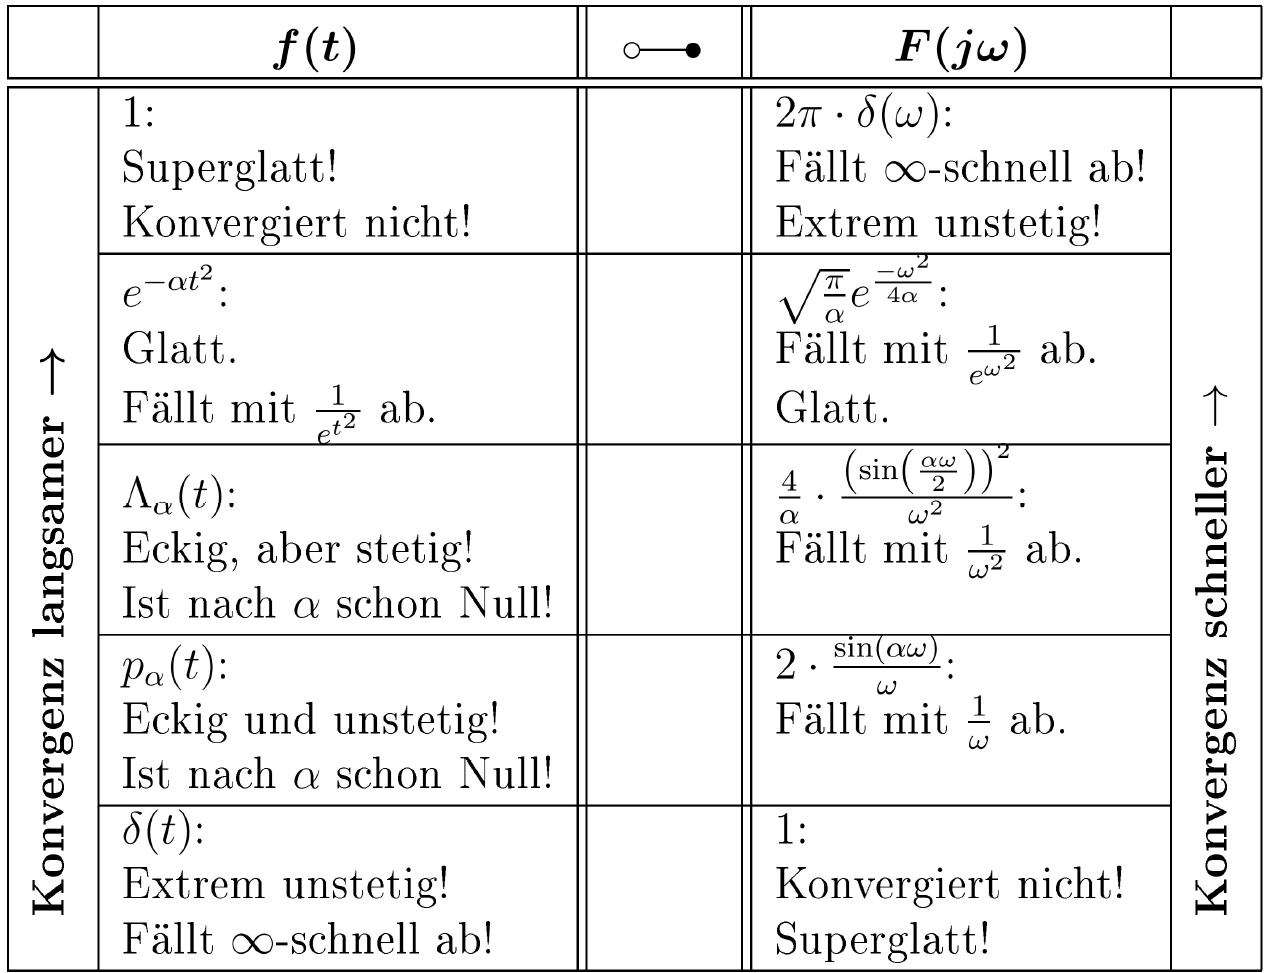
\includegraphics[width=0.7\columnwidth]{images/konvergenzgeschwindigkeit.png}
\end{center}

Im Frequenzbereich passiert das \textbf{duale} zum Zeitbereich!


\subsection{Eigenschaften der Fourier-Transformation}{124-130}

\subsubsection{Übersicht}

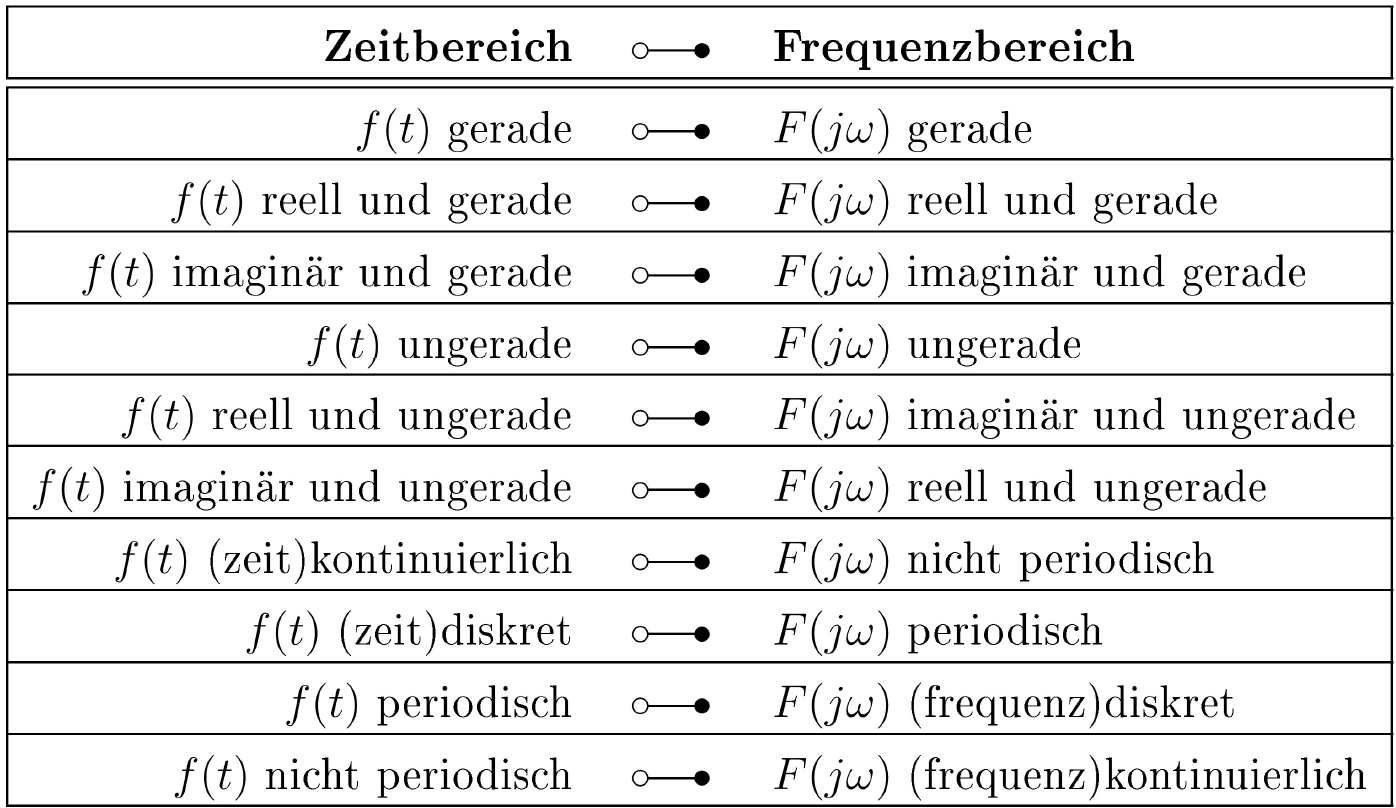
\includegraphics[width=\columnwidth]{images/eigenschaften_fourier_transformation}

\begin{center}
	\begin{tabular}{l c l}
		$f(t)$ reell 		& $\laplace$ 	& $F(-\jimg \omega) = F^*(\jimg \omega)$ konjugiert komplex	\\
		$f(-t) = f^*(t)$ 	& $\laplace$ 	& $F(\jimg \omega)$ reell
	\end{tabular}
\end{center}


\subsubsection{Rechenregeln}

{\renewcommand{\arraystretch}{1.6}
\begin{tabularx}{\columnwidth}{@{}>{\raggedright\arraybackslash}X >{$\displaystyle}c<{$} c >{$\displaystyle}c<{$}@{}}
	\toprule
	\textbf{Eigenschaft} & f(t) & & F(\jimg \omega) \\
	\midrule
	Linearität ($\alpha, \beta \in \mathbb{C}$) 	& \alpha f(t) + \beta g(t) 	& $\laplace$ & \alpha F(\jimg \omega) + \beta G(\jimg \omega) \\
	Ähnlichkeit ($\alpha \in \mathbb{R} \setminus \{0\}$) & f(\alpha t) & $\laplace$ & \frac{1}{|\alpha|} F\Big(\jimg \frac{\omega}{\alpha}\Big) \\
	Zeitumkehrung 					& f(-t) 					& $\laplace$ & F(-\jimg \omega) \\
	Verschiebung Zeit 				& f(t \pm t_0) 				& $\laplace$ & F(\jimg \omega) \, e^{\pm \jimg \omega t_0} \\
	Verschiebung Frequenz 			& f(t) \, e^{\pm \jimg \omega_0 t} & $\laplace$ & F(\jimg(\omega \mp \omega_0)) \\
	Ableitung Zeit ($n \in \mathbb{N}_0$) 	& \frac{d^n f(t)}{dt^n} 	& $\laplace$ & (\jimg \omega)^n F(\jimg \omega) \\
	Ableitung Frequenz ($n \in \mathbb{N}_0$) & t^n f(t) 			& $\laplace$ & \jimg^n \frac{d^n F(\jimg \omega)}{d\omega^n} \\
	Integration Zeit 				& \int_{-\infty}^{t} f(\tau) \, d\tau & $\laplace$ & \frac{F(\jimg \omega)}{\jimg \omega} + F(\jimg 0) \, \pi \delta(\omega) \\
	Faltung Zeit 					& f(t) * g(t) 				& $\laplace$ & F(\jimg \omega) \cdot G(\jimg \omega) \\
	Faltung Frequenz 				& f(t) \cdot g(t) 			& $\laplace$ & \frac{1}{2\pi} F(\jimg \omega) * G(\jimg \omega) \\
	Modulation cos 					& \cos(\alpha t) f(t) 		& $\laplace$ & \tfrac{1}{2} \big[ F(\jimg(\omega - \alpha)) + F(\jimg(\omega + \alpha)) \big] \\
	Modulation sin 					& \sin(\alpha t) f(t) 		& $\laplace$ & \tfrac{1}{2\jimg} \big[ F(\jimg(\omega - \alpha)) - F(\jimg(\omega + \alpha)) \big] \\
	Vertauschung (Dualität) 		& F(\jimg t) 				& $\laplace$ & 2\pi \, f(-\omega) \\
	Dirac-Folge 					& \sum_{n} \delta(t - n t_0) & $\laplace$ & \frac{2\pi}{t_0} \sum_{n} \delta\Big(\omega - n \frac{2\pi}{t_0}\Big) \\
	\bottomrule
\end{tabularx}}

\vspace{0.2cm}

Faltung: $f(t) * g(t) = \int_{-\infty}^{\infty} f(\tau) \, g(t-\tau) \, d\tau$ \qquad Dualität gilt, wenn $f(t) \laplace F(\jimg \omega)$

\subsubsection{Integralbeziehungen}

{\renewcommand{\arraystretch}{2}
\begin{tabularx}{\columnwidth}{@{}>{\raggedright\arraybackslash}X >{$\displaystyle}l<{$}@{}}
	\toprule
	Parseval 			& \int_{-\infty}^{\infty} f(t) \, g^*(t) \, dt = \frac{1}{2\pi} \int_{-\infty}^{\infty} F(\jimg \omega) \, G^*(\jimg \omega) \, d\omega \\
	Bessel (Rayleigh) 	& \int_{-\infty}^{\infty} |f(t)|^2 \, dt = \frac{1}{2\pi} \int_{-\infty}^{\infty} |F(\jimg \omega)|^2 \, d\omega \\
	Anfangswerte 		& f(0) = \frac{1}{2\pi} \int_{-\infty}^{\infty} F(\jimg \omega) \, d\omega \qquad F(\jimg 0) = \int_{-\infty}^{\infty} f(t) \, dt \\
	\bottomrule
\end{tabularx}}


\subsection{AKF und Leistungsdichtespektrum}{132}

\subsubsection{Leistungsdichtespektrum}

Die \textbf{normierte Leistung $\bm{P_n}$} eines \textbf{Leistungssignals $\bm{f(t)}$} kann mit der Hilfe des 
\textbf{Leistungsdichtespektrums $\bm{\Phi(\jimg \omega)}$} beschrieben werden.
$$ \boxed{  P_n = \lim\limits_{T \to \infty} \frac{1}{T} \int\limits_{-T/2}^{T/2} | f(t) |^2 \, \diff t
	= \frac{1}{2 \pi} \int\limits_{-\infty}^{\infty} \Big( \lim\limits_{T \to \infty} \frac{|F(\jimg \omega)|^2}{T} \Big) \, \diff \omega } $$

\vspace{0.2cm}

Der Integrand wird als \textbf{Leistungsdichtespektrums $\bm{\Phi(\jimg \omega)}$} bezeichnet:
$$ \boxed{ \Phi(\jimg \omega) = \lim\limits_{T \to \infty} \frac{|F(\jimg \omega) |^2}{T} } $$

\vspace{0.2cm}

Die \textbf{normierte Leisung $\bm{P_n}$} ist somit:
$$ \boxed{ X^2 = \varphi_{xx}(0) = P_n = \frac{1}{2 \pi}  \int\limits_{- \infty}^{\infty}  \Phi(\jimg \omega) \, \diff \omega } $$


\subsubsection{Energiedichtespektrum}
Analog zum Leistungsdichtespektrum lässt sich für ein \textbf{Energiesignal} (Klasse 1) das 
\textbf{Energiedichtespektrum $\bm{E(\jimg \omega)}$} finden
$$ \boxed{ W_n = \lim\limits_{T \to \infty} \int\limits_{-T/2}^{T/2} |f(t)|^2 \, \diff t = \frac{1}{2 \pi}  \int\limits_{- \infty}^{\infty} |F(\jimg \omega)|^2 \, d\omega } $$

\vspace{0.2cm}

Das \textbf{Energiedichtespektrum $\bm{E(\jimg \omega)}$} ist somit
$$ \boxed{ E(\jimg \omega) = |F(\jimg \omega)|^2 } $$


\subsection{Wiener-Chintschin Theorem}{133}

\subsubsection{Aperiodische Leistungssignale (Klasse 2b)}

Die AKF und das Leistungsdichtespektrum sind ein Fourier-Transformationspaar
$$ \boxed{ \varphi_{xx}(t) = \frac{1}{2 \pi} \int\limits_{- \infty}^{\infty} \Phi(\jimg \omega) \, e^{\jimg \omega t} \, d\omega \, \laplace \, \Phi(\jimg \omega) 
	= \int\limits_{- \infty}^{\infty} \varphi_{xx}(t) \, e^{-\jimg \omega t} \, \diff t } $$


\subsubsection{Periodische Leistungssignale (Klasse 2a) }

$$ \boxed{ \varphi_{xx}(t) = \sum\limits_{k = - \infty}^{\infty} |c_k|^2  \, e^{\jimg \frac{2 \pi k}{T_0} t } \, \laplace \, \Phi(\jimg \omega) 
	= 2 \pi \sum\limits_{k = - \infty}^{\infty}  |c_k|^2 \delta \Big( \omega - \frac{2 \pi k}{T_0} \Big) } $$


\subsubsection{Energiesignale (Klasse 1) }
Die AKF und das Energiedichtespektrum sind ein Fourier-Transformationspaar
$$ \boxed{ \varphi_{xx}(t) = \frac{1}{2 \pi} \int\limits_{- \infty}^{\infty} E(\jimg \omega) \, e^{\jimg \omega t} \, d\omega \, \laplace \, E(\jimg \omega)
	= \int\limits_{- \infty}^{\infty} \varphi_{xx}(t) \, e^{-\jimg \omega t} \, \diff t } $$